\subsection{Authentication Page (Tom)}

The authentication page is the entry point to the system and as such we designed it very carefully. It exists in 3 versions:
\begin{enumerate}
  \item A default view:
  	\subitem 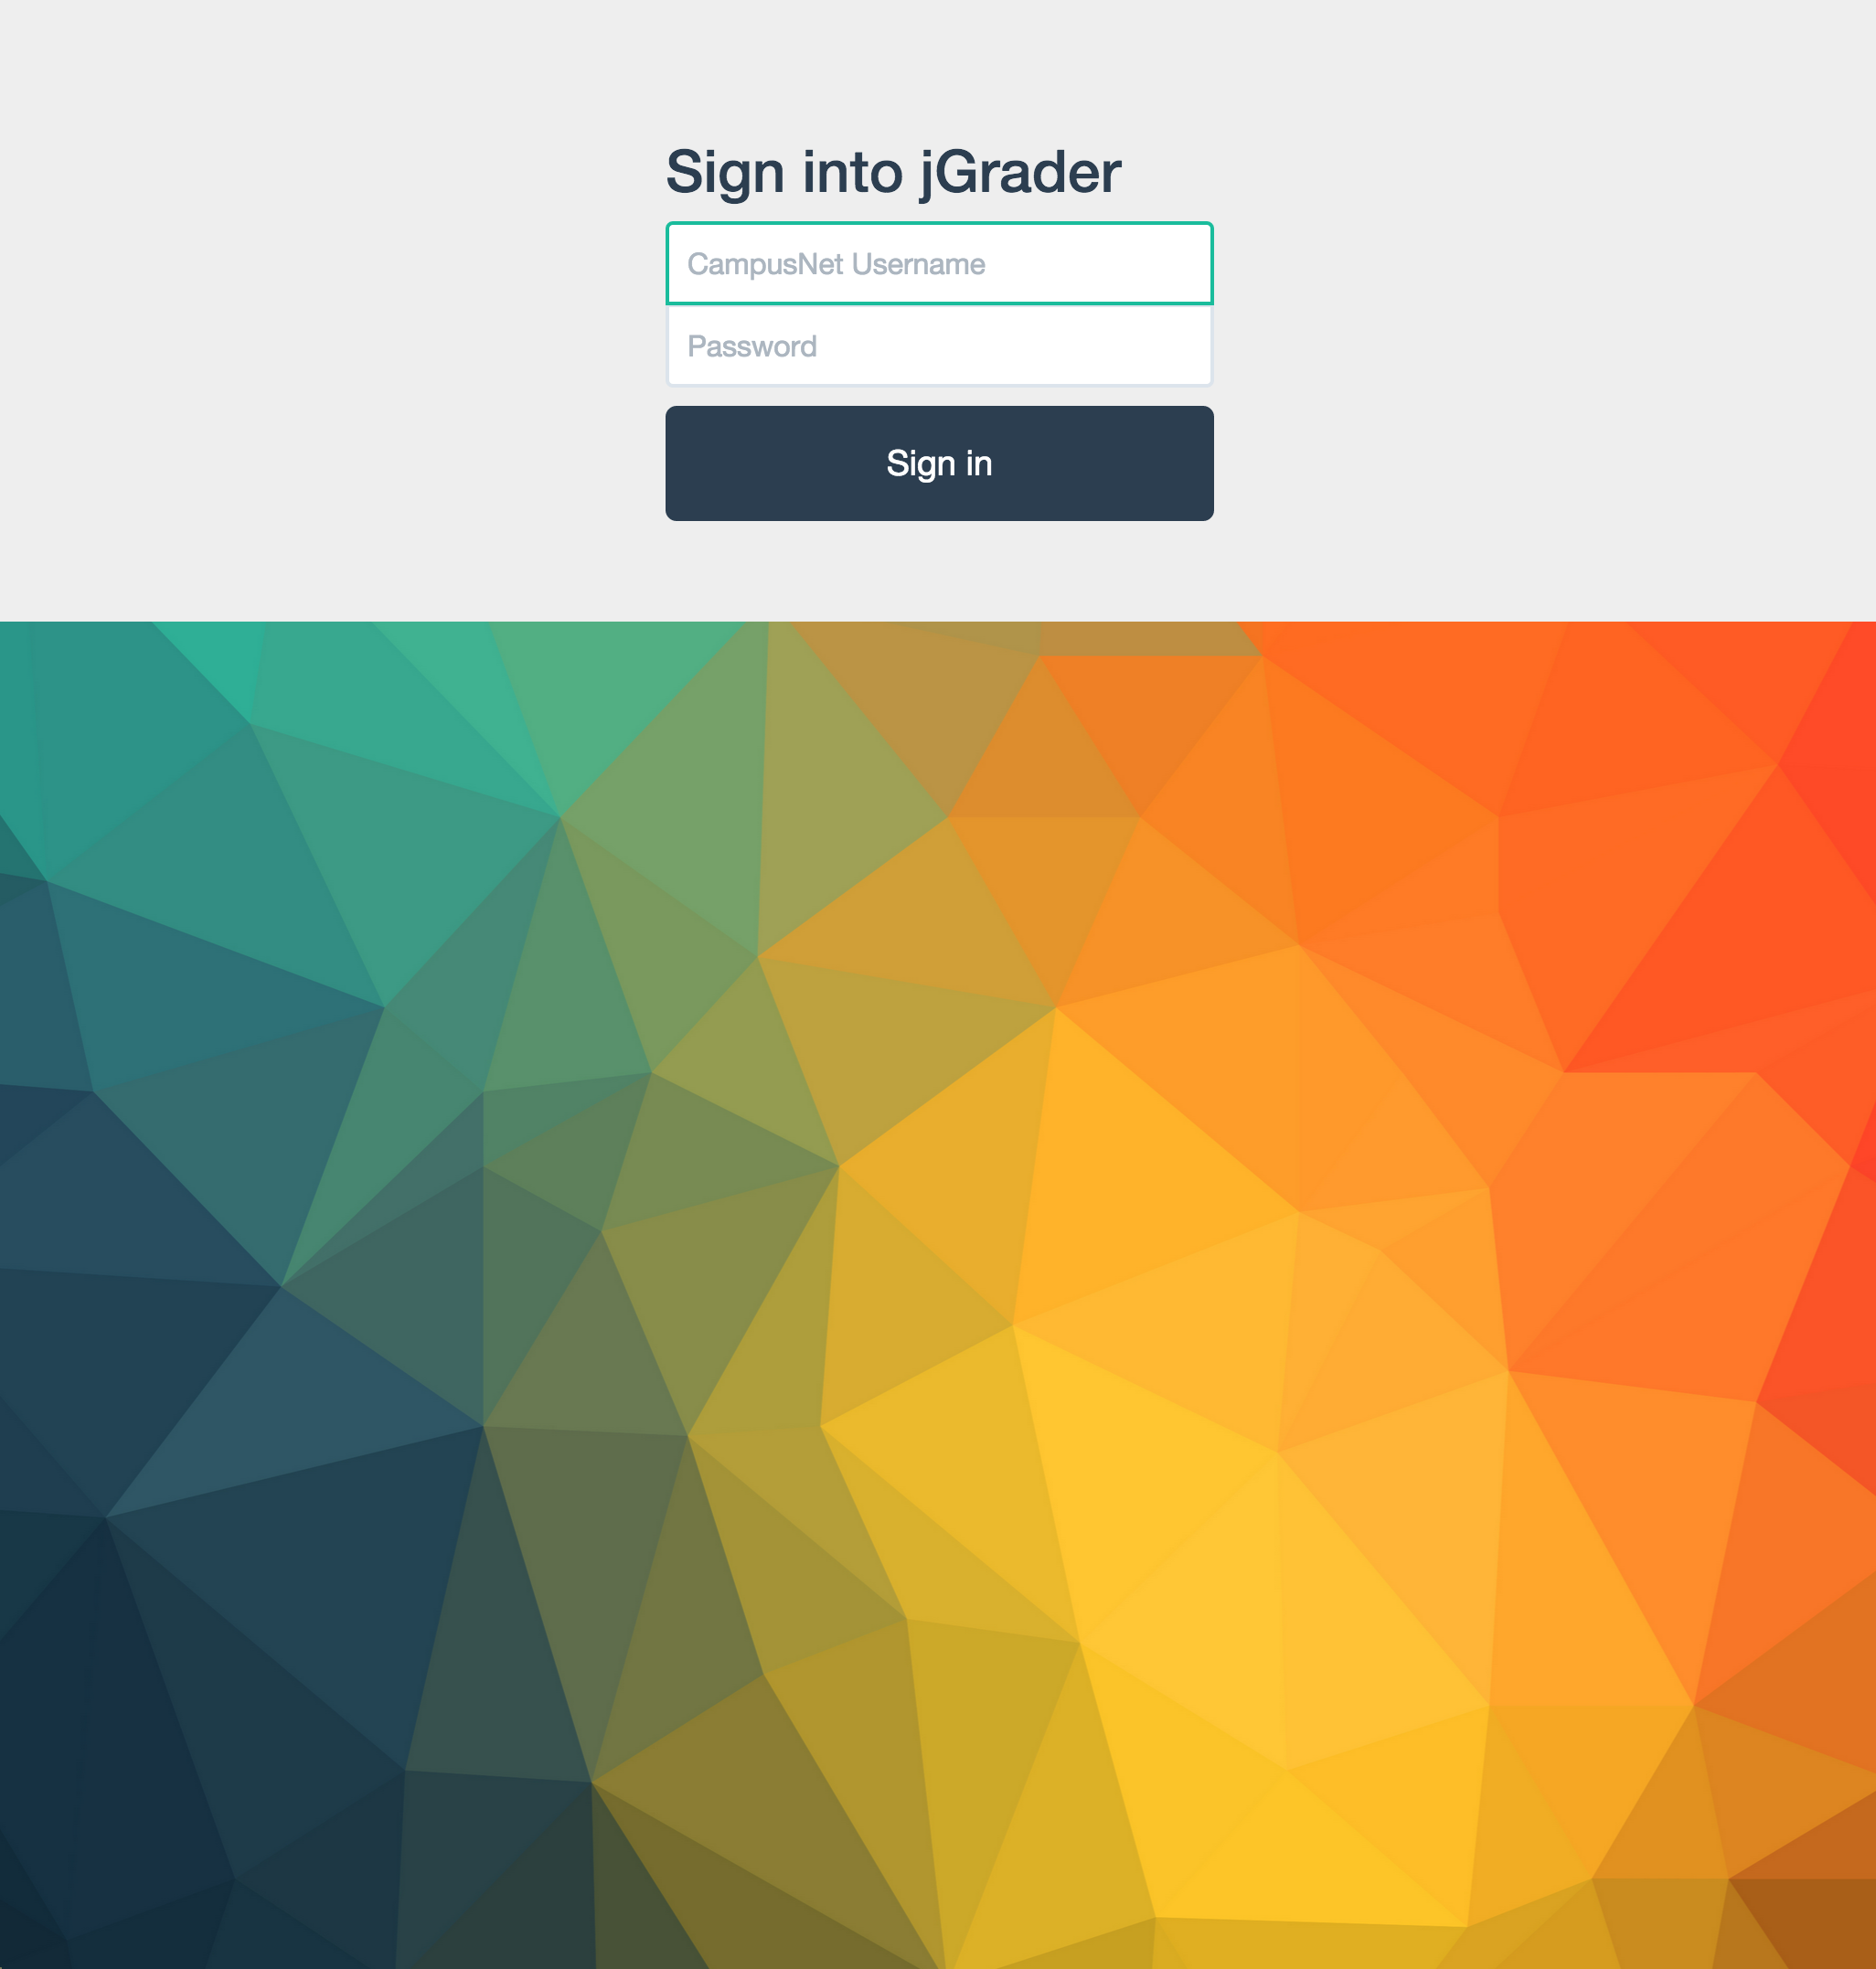
\includegraphics[width=.55\textwidth]{screenshots/SignIn.png}
  \item A view that appears if the user enters an incorrect password: 
   	\subitem 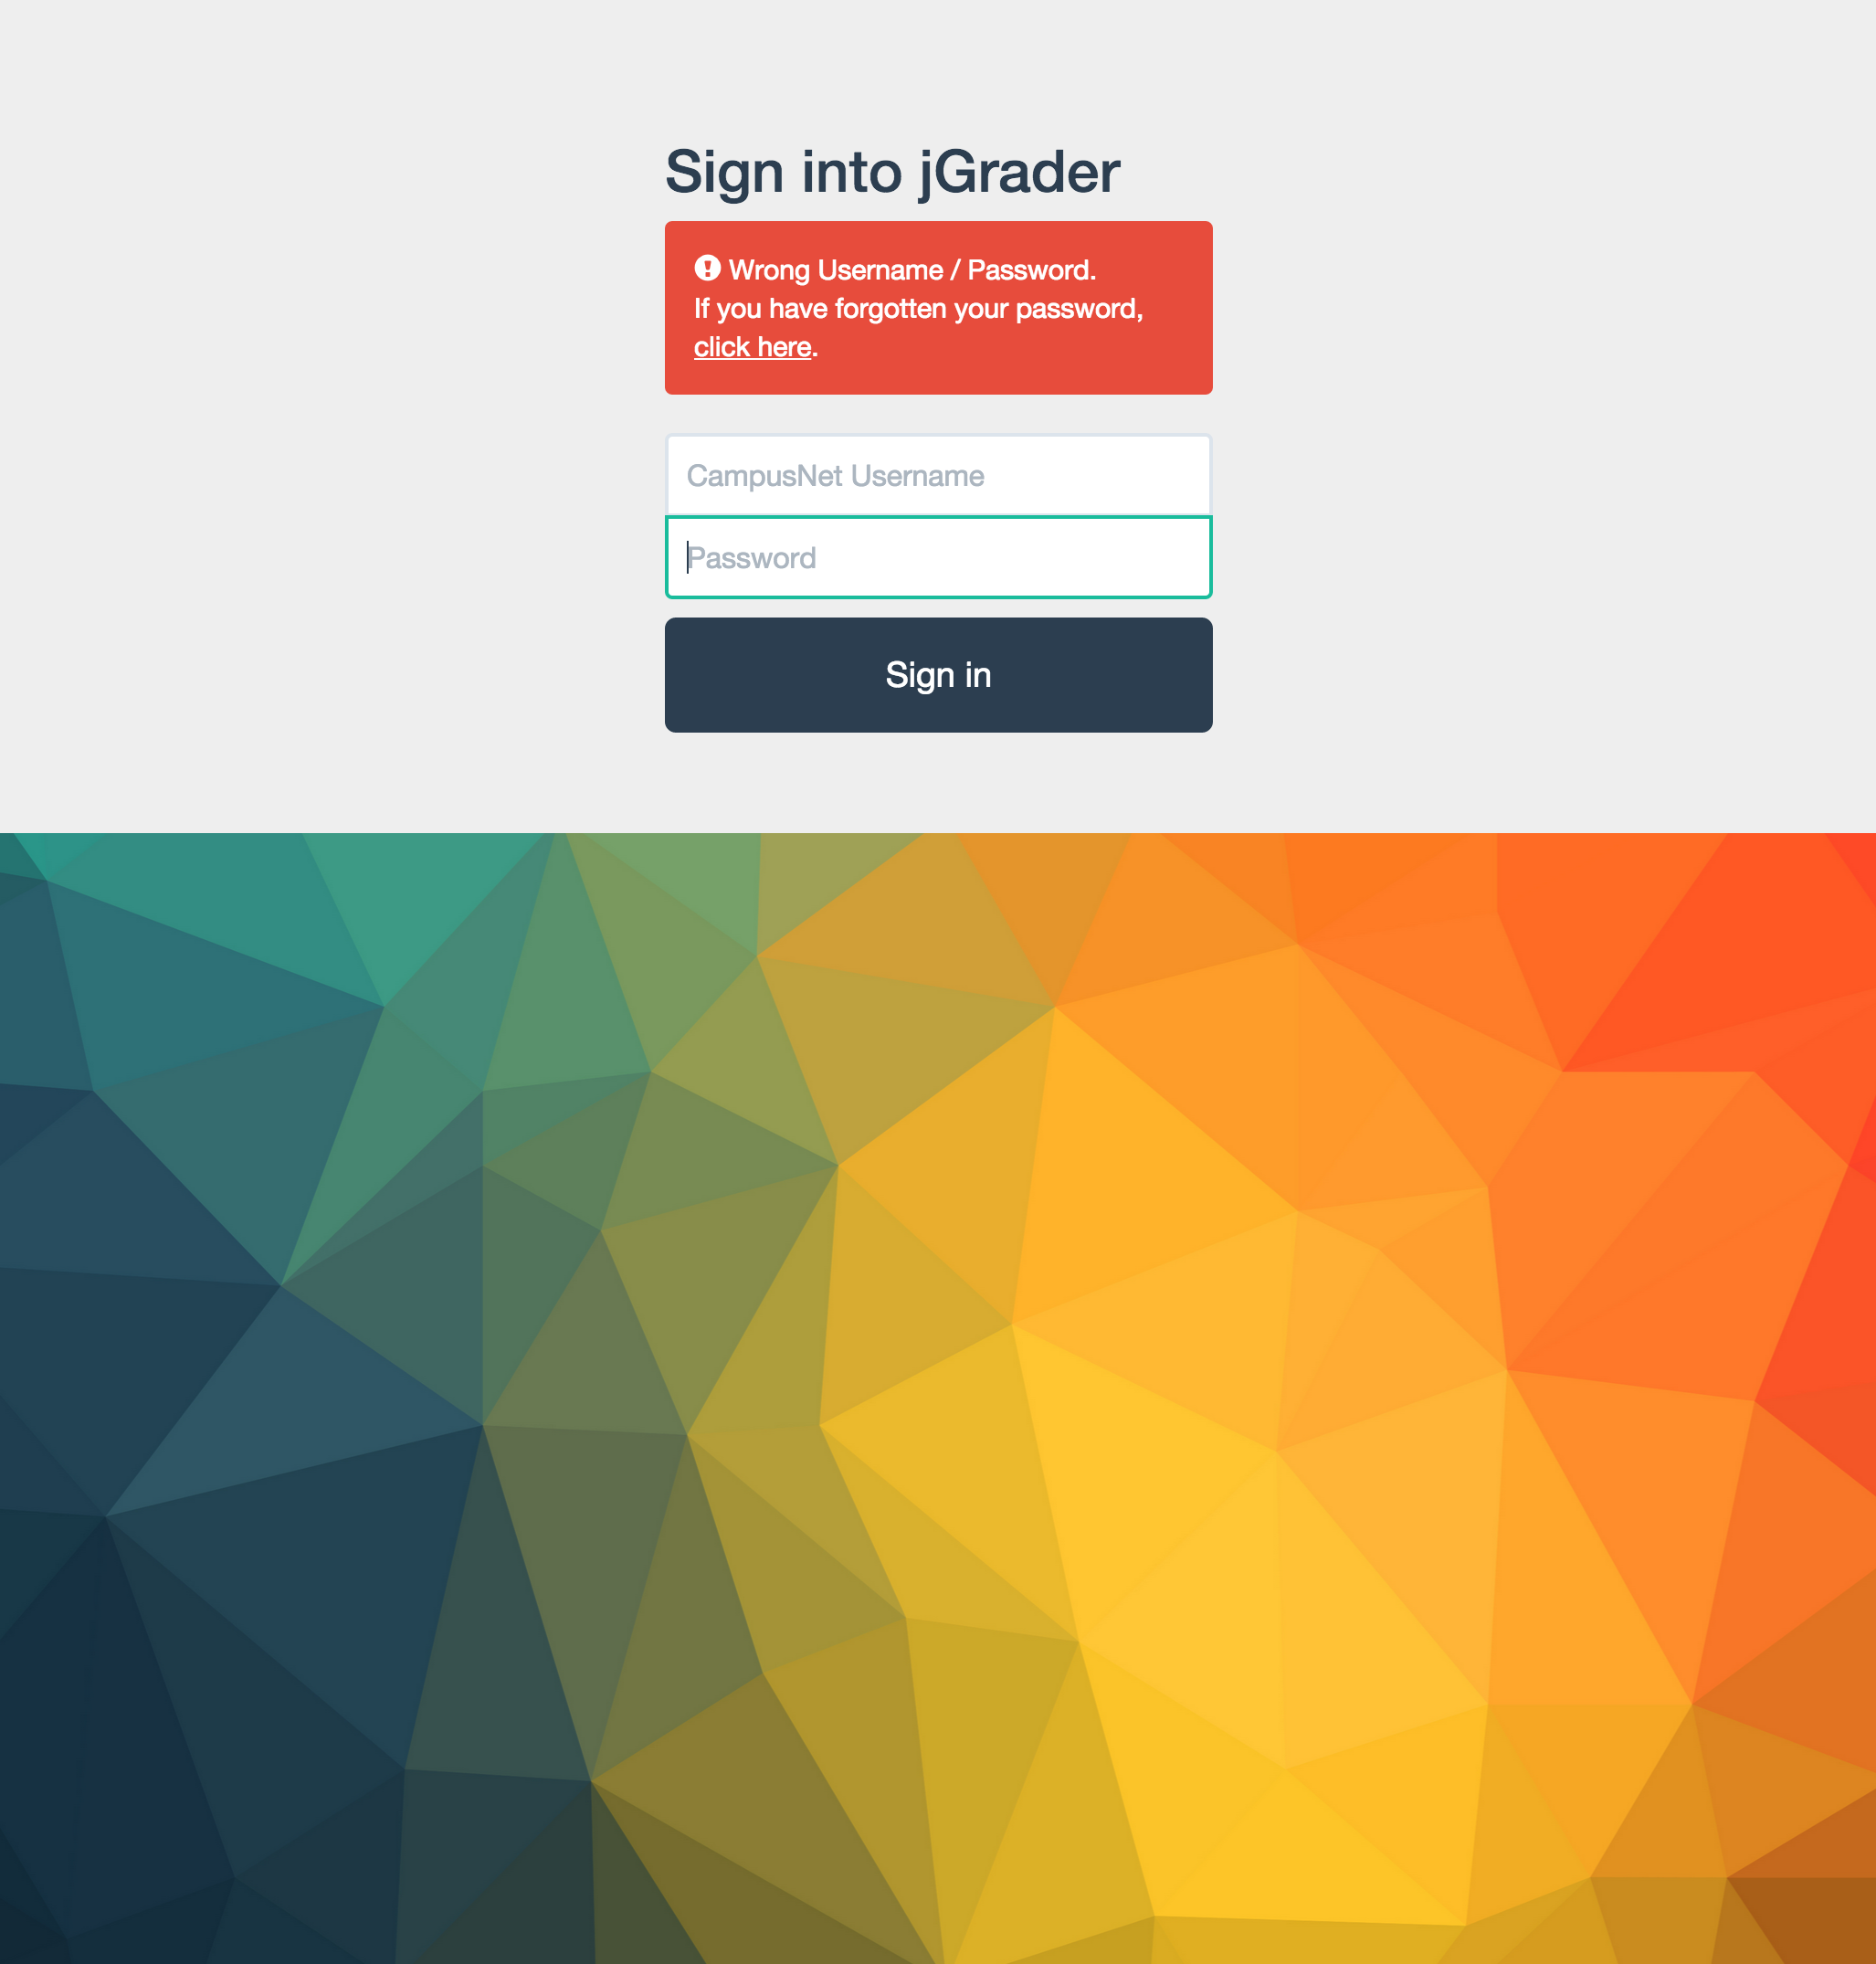
\includegraphics[width=.55\textwidth]{screenshots/WrongPW.png}
  \item A view that appears if the user just logged out: 
   	\subitem 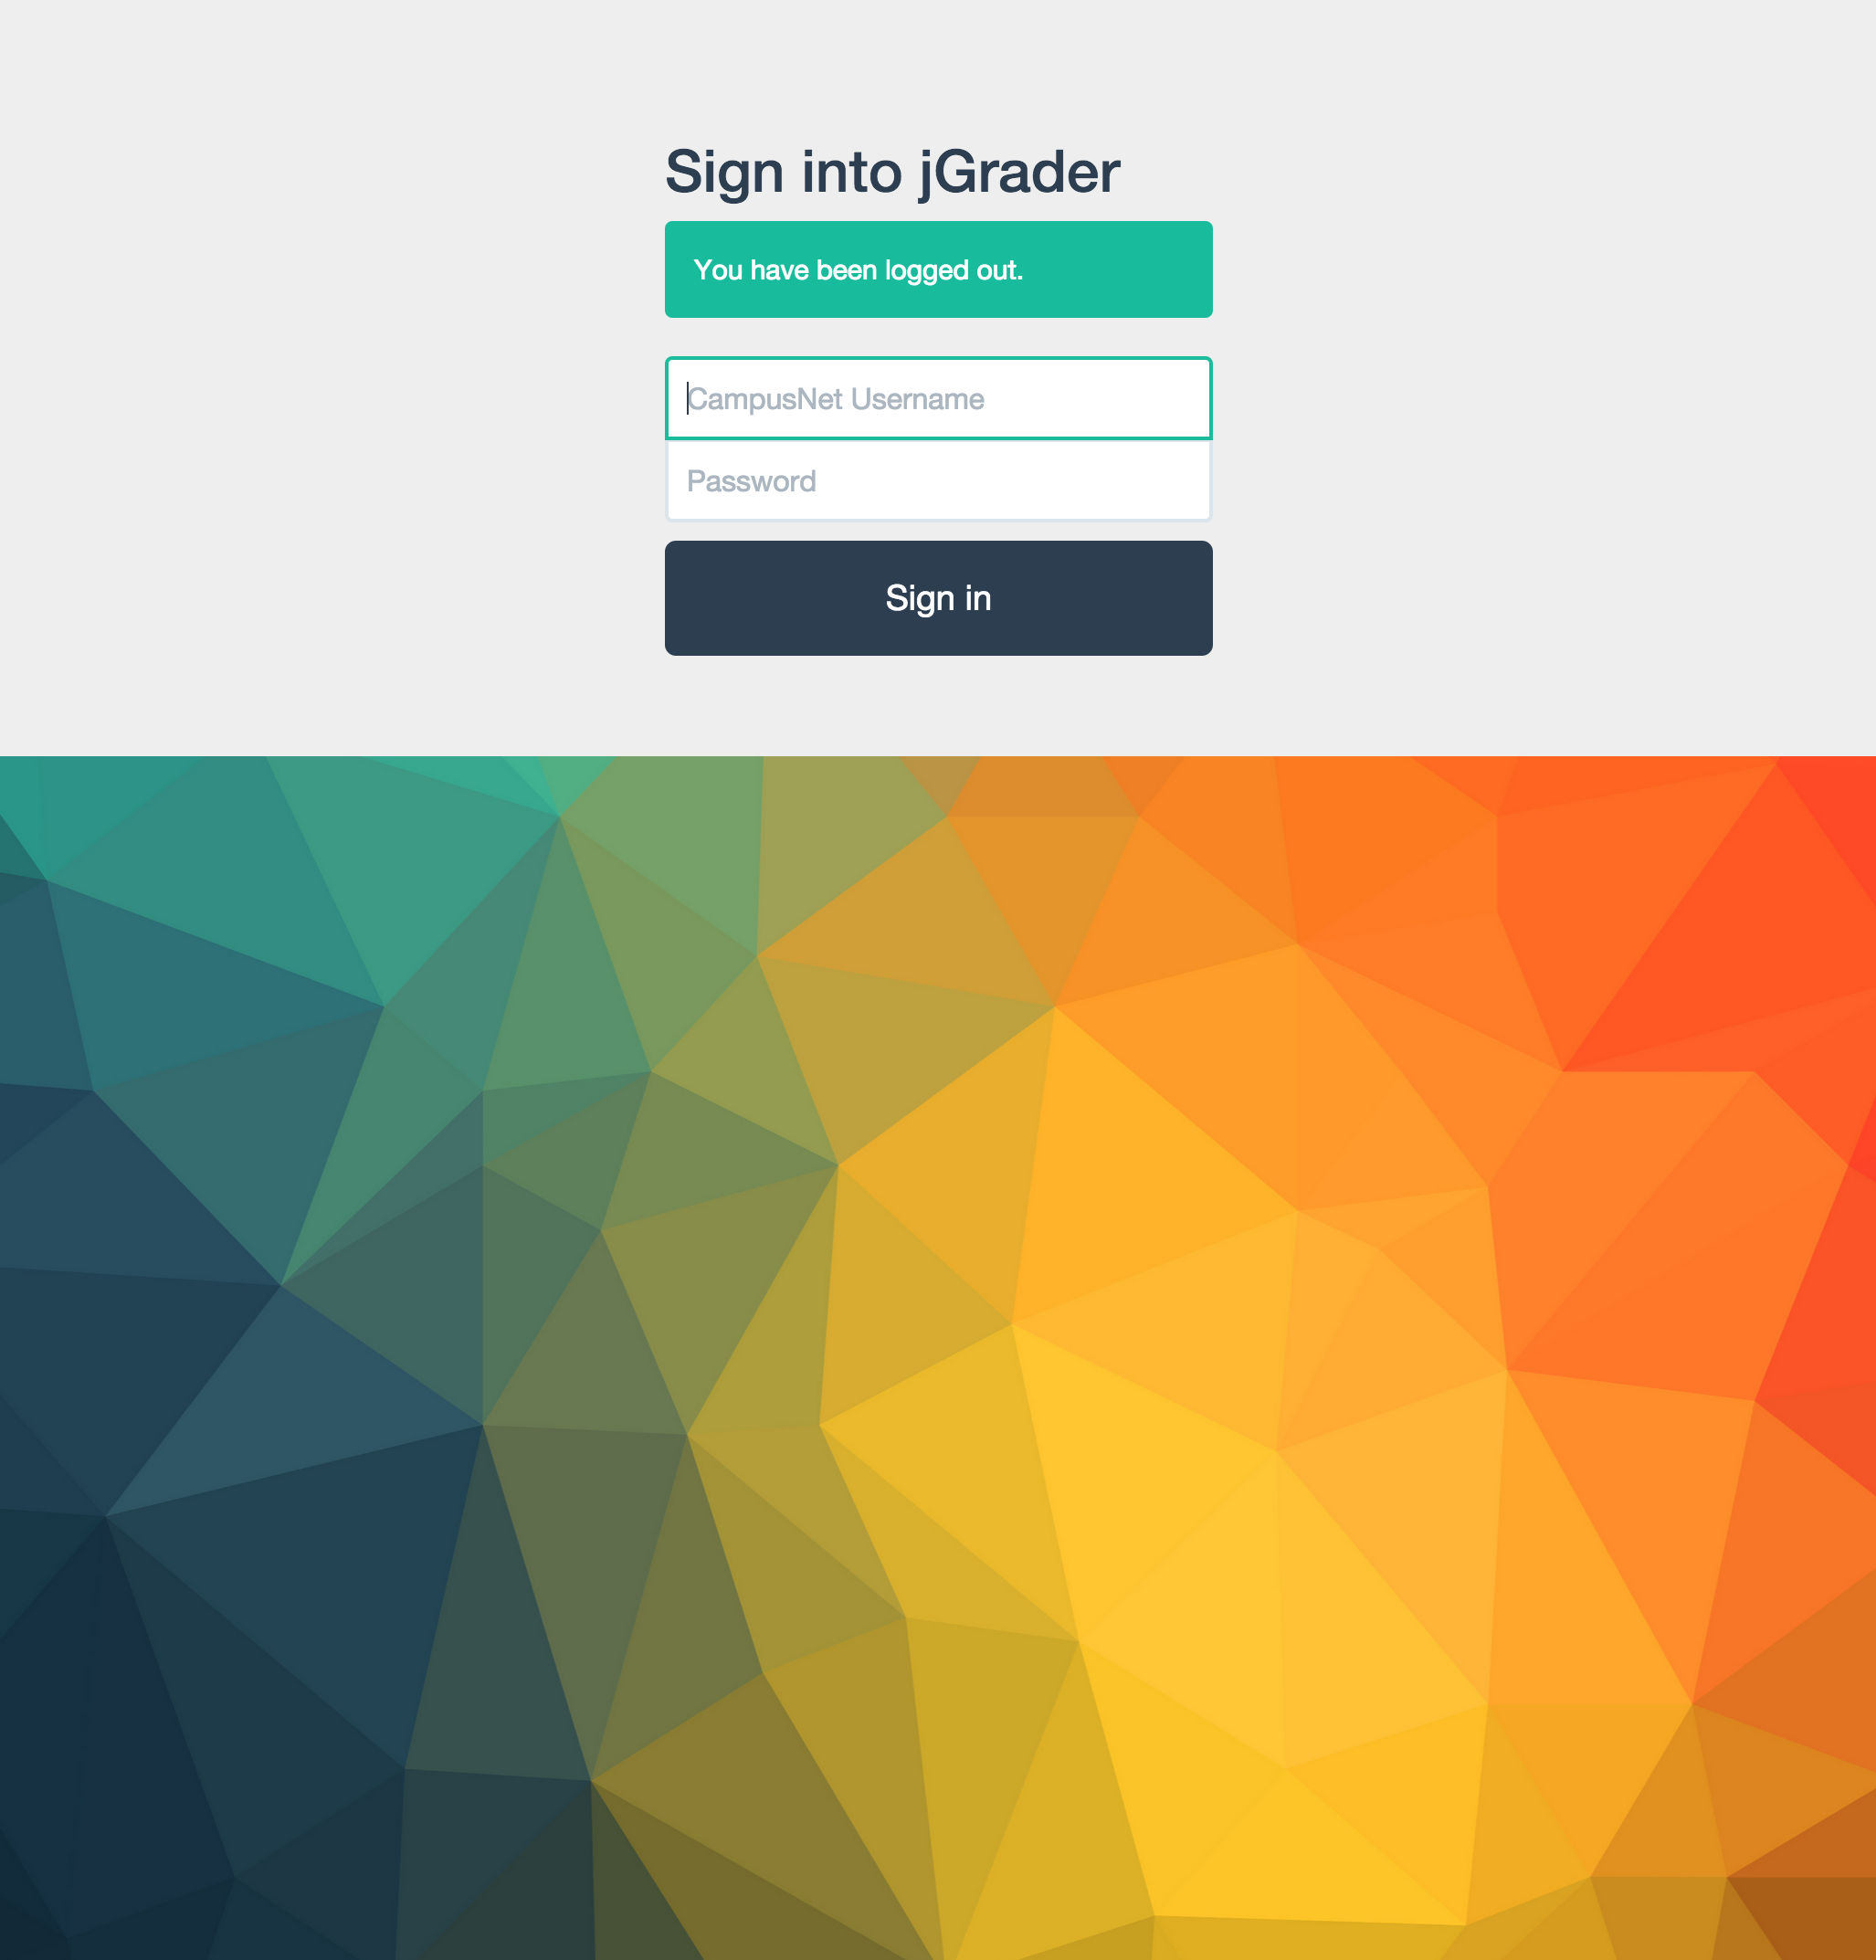
\includegraphics[width=.55\textwidth]{screenshots/LogOut.png}
\end{enumerate}
\newpage

Each of the versions has the same basic layout. The only real content of the page is centered. It contains a heading, input elements for username and password as well as a submit button. We designed it this way because we want to draw the users attention to its use, being as minimalistic as possible. However because it is the first contact any user has with the system we wanted to leave an impression and added a colorful background image.

When the user accesses the sign in page for the first time, the keyboard automatically focuses the username field. This makes it easy for the user to sign into the system. When the user enters a wrong password they end up the second version of the page, which in addition has an error message and a forgot password link. The keyboard is automatically focused on the password field so the user can quickly re-enter the password since it is more likely that the password, and not the username, is incorrect. To further speed up loggin in, the username field keeps the value entered in the first sign in attempt.

During (paper) prototype testing a tester mentioned that it would be convenient to have reset password functionality, so we added a link for it.  On the linked page the user can enter their username and then gets an email with a link to reset the password\footnote{Because this is simply a prototype only the form is implemented, not the actual mail being sent. We also do not have a layout for the reset password page. If this system were to be used at Jacobs, the reset link might be removed because CampusNet accounts are used and we are not capable of resetting CampusNet accounts without Campus IT.}. This page does not have the username pre-entered or an auto-focus functionality because we want to prevent abuse of the system.

The third version of the authentication is shown after the user signs out of the system. It contains a small message to ensure that the user knows they have been signed out. Furthermore if auto-focuses the username field to enable the user to quickly sign in again. An earlier version did not contain a sign in form but only a message that the user had been logged out, however this was criticized during paper prototype testing. 
